\documentclass[12pt, a4paper]{article}
\edef\restoreparindent{\parindent=\the\parindent\relax}
\usepackage{amsmath, amssymb}
\usepackage[UKenglish]{babel}
\usepackage[bibstyle=ieee, dashed=false, sorting=nty]{biblatex}
\usepackage[labelfont=bf]{caption}
\usepackage{colortbl}
\usepackage{csquotes}
\usepackage{enumitem}
\usepackage{fancyhdr}
\usepackage{float}
\usepackage[top=25mm, right=25mm, bottom=25mm, left=25mm]{geometry}
\usepackage{graphicx}
\usepackage{hyperref}
\usepackage[capitalise, nameinlink, noabbrev]{cleveref}
\usepackage{listings}
\usepackage{longtable}
\usepackage{minted}
\usepackage{microtype}
\usepackage{multirow,multicol}
\usepackage{parskip}
\usepackage{subcaption}
\usepackage{tikz, pgfplots}
\usepackage{tcolorbox}
\usepackage{xcolor}

\restoreparindent

\pagestyle{fancy}
\fancyhead[L]{COM4521}
\fancyhead[C]{Assignment: N-body Simulation}
\fancyhead[R]{Part 2}
\setlength{\headheight}{15pt}

\usemintedstyle{vs}

% colours used in table
\definecolor{lightgray}{HTML}{E3E3E3}
\definecolor{green}{HTML}{B7E1CD}

\pgfplotsset{compat=newest}
\usepgfplotslibrary{units}
\usepgfplotslibrary{groupplots}

\let\oldcref\cref
\renewcommand{\cref}[1]{\textbf{\oldcref{#1}}}

\addbibresource{references.bib}

\begin{document}

\renewcommand{\baselinestretch}{1.3}\normalsize
\tableofcontents
\renewcommand{\baselinestretch}{1.0}\normalsize
\newpage

% ======================================================
\section{Introduction}

\subsection{Development and Benchmark Environment} \label{subsec:development_environment}
\begin{enumerate}
  \item Operating system: Windows 10 64-bit
  \item CPU: Intel\textsuperscript{\textregistered} Core\texttrademark\ i7-7700HQ, 4 cores, 8
  threads
  \item RAM: 16GB DDR4-2400MHz
  \item GPU: Geforce GTX 1060 (Mobile)
    \begin{enumerate}[label=\alph*.]
      \item \makebox[10cm][l]{CUDA compute capability} : 6.1
      \item \makebox[10cm][l]{(10) multiprocessors, (128) CUDA cores / MP} : 1280 CUDA cores
      \item \makebox[10cm][l]{Total amount of global memory} : 6144 MBytes
      \item \makebox[10cm][l]{Total amount of constant memory} : 65536 bytes
      \item \makebox[10cm][l]{Total amount of shared memory per block} : 49152 bytes
      \item \makebox[10cm][l]{Total number of registers available per block} : 65536
      \item \makebox[10cm][l]{Maximum number of threads per multiprocessor} : 2048
      \item \makebox[10cm][l]{Maximum number of threads per block} : 1024
      \item \makebox[10cm][l]{Max dimension size of a thread block (x, y, z)} : (1024, 1024, 64)
    \end{enumerate}
\end{enumerate}

The GPU information is obtained through the \texttt{deviceQuery} sample provided by NVIDIA
\cite{deviceQuery}. Some of the common properties are listed here as a reference for the development
process.

\subsection{Baseline Implementation (Naive Implementation)}
The baseline implementation is a basic conversion of the CPU code to GPU code without including any
further optimisation techniques. It is used as a baseline for measuring the effectiveness of
different optimisations introduced during the iterative refinement.

The following implementation techniques are selected as the baseline implementation.
\begin{enumerate}
  \item \textbf{Parallelisation Method:} Parallelise each body (N threads)
  \item \textbf{Data Layout Structure:} Array of Structure
  \item \textbf{Memory cache:} Global memory
  \item \textbf{Threads per block}: 32 (\texttt{THREADS\_PER\_BLOCK})
  \item \textbf{Grid Dimension}: 1 dimension. Blocks per grid is rounded up if \textbf{N} or
  \textbf{D} is not a multiple of \texttt{THREADS\_PER\_BLOCK}.
\end{enumerate}

\subsubsection{Kernel 1: Compute Force}
This kernel is responsible for calculating the summation of force for each n-body. Since the
baseline implementation is using \textbf{N} threads, there will be a single \mintinline{c}{for} loop
inside the kernel to calculate the summation part. Each thread in a block represents a single body.

\begin{listing}[ht]
  \begin{minted}[linenos, frame=lines, framesep=2mm, fontsize=\footnotesize]{cuda}
__global__ void compute_force(...) {
    const unsigned int i = blockIdx.x * blockDim.x + threadIdx.x;

    if (i < N) {
        float local_sum_x = 0, local_sum_y = 0;

        // Summation of forces for the current n-body
        for (unsigned int j = 0; j < N; ++j) { ... }

        d_force_sum[i].x = local_sum_x;
        d_force_sum[i].y = local_sum_y;
    }
}
  \end{minted}
  \caption{CUDA kernel for computing the summation of force for each n-body.}
\end{listing}

\subsubsection{Kernel 2: Update Body}
After the summation of force has been computed for each n-body, the result is then passed to the
\texttt{update\_body} kernel. The \texttt{update\_body} will update the position and velocity of
each body, then it will calculate the new cell of the body and increase the count. Race condition is
prevented by using CUDA atomic function \cite{atomic_func}, as shown in line 11 of
\cref{listing:baseline_update_body}.

\begin{listing}[ht]
  \begin{minted}[linenos, frame=lines, framesep=2mm, fontsize=\footnotesize]{cuda}
__global__ void update_body(...) {
    const unsigned int i = blockIdx.x * blockDim.x + threadIdx.x;

    if (i < N) {
        // Update x, y, vx, vy

        // Do not update `d_activity_map` if n-body is out of grid area
        if (cell < grid_size) {
            atomicAdd(&d_activity_map[cell], 1); // Prevent race condition
        }
    }
}
  \end{minted}
  \caption{CUDA kernel for updating each body.}
  \label{listing:baseline_update_body}
\end{listing}

\subsubsection{Kernel 3: Normalising Activity Map}
The last step is to normalise the activity map. This kernel is relatively simpler. Each thread
represents a cell in the activity map.
\begin{listing}[ht]
  \begin{minted}[linenos, frame=lines, framesep=2mm, fontsize=\footnotesize]{cuda}
__global__ void normalise_activity_map(...) {
    const unsigned int i = blockIdx.x * blockDim.x + threadIdx.x;

    // `grid_size` and `normalising_factor` are runtime calculated constants
    if (i < grid_size) {
        d_activity_map[i] *= normalising_factor;
    }
}
  \end{minted}
  \caption{CUDA kernel for normalising the activity map.}
\end{listing}

\pagebreak
\subsection{Fixed Variables of Benchmark}
\subsubsection{Number of Simulation Iterations}
Fixed arguments: $\textbf{N} =$ 5000, $\textbf{D} =$ 10

\begin{figure}[ht]
  \centering
  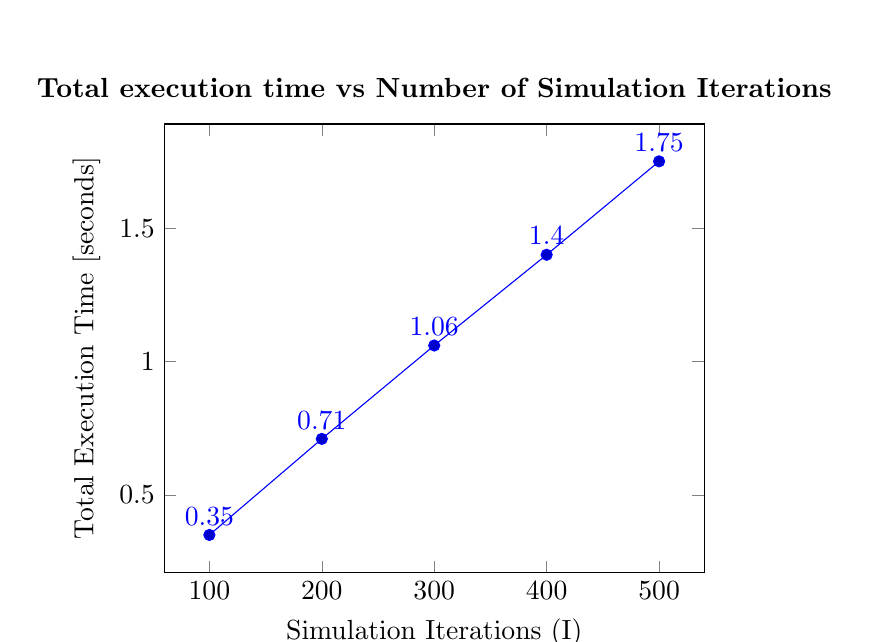
\begin{tikzpicture}
    \begin{axis}[nodes near coords, y unit=seconds, xlabel=Simulation Iterations (I), ylabel=Total
      Execution Time, title=\textbf{Total execution time vs Number of Simulation Iterations}]
      \addplot coordinates {(100, 0.35) (200, 0.71) (300, 1.06) (400, 1.40) (500, 1.75)};
    \end{axis}
  \end{tikzpicture}
  \caption{Relationship between the total execution time and number of simulation iterations in CUDA mode.}
  \label{figure:simulation_iterations}
\end{figure}

As shown in \cref{figure:simulation_iterations}, the total execution time is \textbf{directly
proportional} to the number of simulation iterations. The value of \textbf{I} should only affect the
total execution time proportionally, but not the simulation performance. Hence, \textbf{I} is
excluded from the benchmark variable.

\subsubsection{Number of Runs per Benchmark}
Each benchmark will be run 10 times to produce an average execution time. This is to minimise the
margin of error caused by uncontrollable environment variables.

\subsection{Baseline Performance} \label{subsec:baseline_performance}
\subsubsection*{\underline{Benchmark on Number of Bodies (N)}}
\textbf{Fixed arguments:} $\textbf{D} =$ 10, $\textbf{I} =$ 100
\renewcommand{\arraystretch}{1.3}
\begin{longtable}{|c|c|c|}
  \hline \endfirsthead \rowcolor{lightgray}
  N     & Average Execution Time of 10 runs (seconds) \\ \hline
  10000 & 0.729                                       \\
  20000 & 2.863                                       \\
  30000 & 6.460                                       \\
  40000 & 11.494                                      \\
  50000 & 17.990                                      \\ \hline
  \caption{Baseline performance of program over various values of \textbf{N}.}
  \label{table:baseline_n}
\end{longtable}
\renewcommand{\arraystretch}{1}

\subsubsection*{\underline{Benchmark on Activity Grid Dimension (D)}}
\textbf{Fixed arguments:} $\textbf{N} =$ 1024, $\textbf{I} =$ 100
\renewcommand{\arraystretch}{1.3}
\begin{longtable}{|c|c|c|}
  \hline \endfirsthead \rowcolor{lightgray}
  D     & Average Execution Time of 10 runs (seconds) \\ \hline
  1000  & 0.087                                       \\
  2000  & 0.135                                       \\
  5000  & 0.468                                       \\
  10000 & 1.658                                       \\
  15000 & 3.620                                       \\ \hline
  \caption{Baseline performance of program over various values of \textbf{D}.}
  \label{table:baseline_d}
\end{longtable}
\renewcommand{\arraystretch}{1}

\subsection{Baseline Profiling on Visual Profiler}
This section summarises the issues of baseline implementation reported by Visual Profiler. Detailed
analysis results will be shown and discussed in other relevant sections. The profiling session is
run with arguments: $\textbf{N} =$ 10000, $\textbf{D} =$ 10, $\textbf{I} =$ 100.

\subsubsection{Analysis Results} \label{subsubsec:baseline_analysis_results}
\begin{enumerate}
  \item Data movement and concurrency
    \begin{enumerate}
      \item Low Memcpy/Kernel Overlap
      \item Low Kernel Concurrency
      \item Low Memcpy Throughput
    \end{enumerate}

  \item Compute Utilisation
    \begin{enumerate}
      \item Low Multiprocessor Occupancy (21.7\% average)
    \end{enumerate}

  \item Kernel Performance
    \begin{enumerate}
      \item Low Global Memory Load Efficiency (18.8\% average)
      \item Low Global Memory Store Efficiency (17.4\% average)
    \end{enumerate}
\end{enumerate}

For 1(a) and 1(c), the issue is unavoidable as the program only needs to do the \texttt{cudaMemcpy}
once before the \texttt{step()} function to transfer the host n-bodies to device. For 1(b), the
kernels \texttt{update\_body} and \texttt{normalise\_activity\_map} have data dependencies on the
previous kernel, so they cannot be executed in parallel.

For 2 and 3, they can be improved with the help of guided analysis. Therefore, the iterative
improvement of the code will try to follow the guided analysis to identify the main bottleneck of
the program and optimise it.

\subsubsection{Kernel Optimisation Priorities}
\begin{figure}[H]
  \centering
  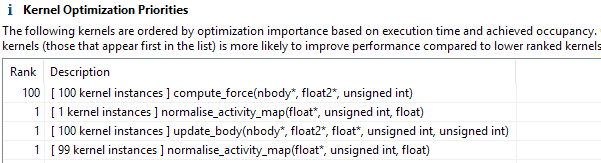
\includegraphics[width=0.75\textwidth]{images/baseline_kernel_optimisation_priorities.png}
  \caption{Kernel optimisation priorities of baseline implementation.}
  \label{figure:baseline_kernel_optimisation_priority}
\end{figure}

As shown in \cref{figure:baseline_kernel_optimisation_priority}, the kernel \texttt{compute\_force}
has the top priority. Therefore, optimisations will be prioritised for the \texttt{compute\_force}
kernel.

\subsubsection{Kernel Analysis: Compute Force}
\begin{figure}[H]
  \centering
  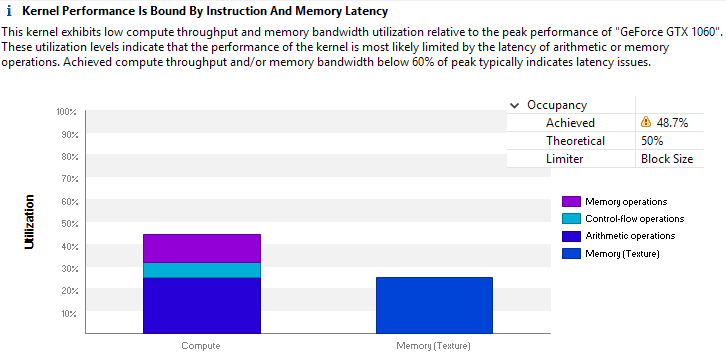
\includegraphics[width=0.9\textwidth]{images/baseline_kernel_analysis_compute_force.png}
  \caption{Kernel analysis of \texttt{compute\_force}.}
  \label{figure:baseline_kernel_analysis_compute_force}
\end{figure}

As shown in \cref{figure:baseline_kernel_analysis_compute_force}, the kernel \texttt{compute\_force}
has low compute and memory utilisation. The occupancy is also limited by the block size of 32.

\subsection{Summary}
\noindent Problems:
\begin{enumerate}
  \item \textbf{Low compute utilisation:} Computation can be improved by reducing the instruction
  dependency and avoid heavy floating point instructions.
  \item \textbf{Low memory utilisation:} Inefficient global memory load and store. It could be
  improved by using constant, read-only, and shared memory to reduce the global load / store
  instructions.
  \item \textbf{Low occupancy and high latency:} This is likely to be caused by the small block
  size. Increasing the block sizes may improve the latency.
\end{enumerate}

% ======================================================
\section{Improving Latency and Occupancy}
According to \cref{figure:baseline_kernel_analysis_compute_force}, Visual Profiler suggests that the
kernel performance is currently limited by latency. Therefore, this optimisation is performed first.

\subsection{Increase the Block Size}
As shown in \cref{figure:latency_analysis_32_threads_per_block}, 32 threads per block is not enough
to fully utilise the device. Moreover, the block  size is also too small to hide the latency of
memory instructions.
\begin{figure}[ht]
  \centering
  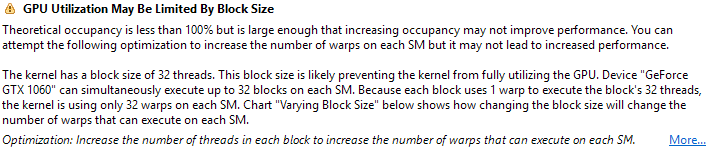
\includegraphics[width=\textwidth]{images/latency_analysis_32_threads_per_block.png}
  \caption{Visual Profiler suggesting a larger block size.}
  \label{figure:latency_analysis_32_threads_per_block}
\end{figure}

\renewcommand{\arraystretch}{1.3}
\begin{longtable}{|c|c|c|c|c|c|}
  \hline \endfirsthead & \multicolumn{5}{c|}{Total Execution Time (seconds)} \\ \cline{2-6}
  \multirow{-2}{*}{Value} & 32 (baseline) & 64 & 128 & 256 & 512 \\ \hline
  \rowcolor{lightgray}\multicolumn{6}{|c|}{\textbf{Number of Bodies (N)}} \\ \hline
  1024  & 0.087  & 0.081  & 0.072  & 0.072  & 0.073  \\
  2048  & 0.154  & 0.155  & 0.144  & 0.144  & 0.144  \\
  4096  & 0.401  & 0.297  & 0.287  & 0.287  & 0.287  \\
  10000 & 0.729  & 0.735  & 0.729  & 0.732  & 0.740  \\
  20000 & 2.863  & 1.863  & 1.849  & 1.862  & 1.873  \\
  30000 & 6.460  & 5.397  & 5.347  & 5.014  & 5.060  \\
  40000 & 11.494 & 7.402  & 7.341  & 7.377  & 7.447  \\
  50000 & 17.990 & 13.397 & 13.283 & 12.845 & 12.786 \\ \hline
  \textbf{Average speedup} & \textbf{-} & \textbf{1.25} & \textbf{1.29} & \textbf{1.31} &
  \textbf{1.30} \\ \hline
  \rowcolor{lightgray}\multicolumn{6}{|c|}{\textbf{Activity Grid Dimension (D)}} \\ \hline
  1000  & 0.087 & 0.080 & 0.079 & 0.080 & 0.080 \\
  2000  & 0.135 & 0.108 & 0.103 & 0.104 & 0.104 \\
  5000  & 0.468 & 0.299 & 0.267 & 0.268 & 0.269 \\
  10000 & 1.658 & 0.983 & 0.855 & 0.854 & 0.861 \\
  15000 & 3.620 & 2.124 & 1.835 & 1.832 & 1.847 \\ \hline
  \textbf{Average speedup} & \textbf{-} & \textbf{1.46} & \textbf{1.62} & \textbf{1.61} &
  \textbf{1.60} \\ \hline
  \caption{Performance comparison of different number of threads per block.}
  \label{table:block_size}
\end{longtable}
\renewcommand{\arraystretch}{1}

According to the results in \cref{table:block_size} and taking the margin of error into account,
128, 256, and 512 threads per block give the best overall performance improvements. At this stage,
it is decided to set the threads per block to 256. After further optimisations have been made, the
threads per block might need to be changed accordingly.

\subsection{Summary}
\begin{figure}[ht]
  \centering
  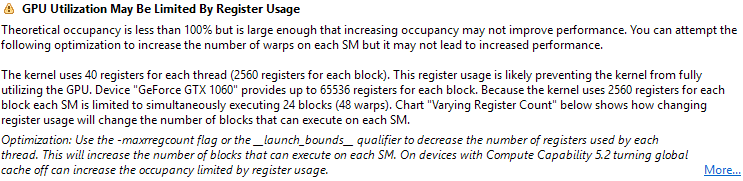
\includegraphics[width=\textwidth]{images/256_threads_per_block.png}
  \caption{Kernel analysis of \texttt{compute\_force} after increasing block size to 256.}
  \label{figure:latency_analysis_256_threads_per_block}
\end{figure}

After increasing the threads per block to 256, both compute and memory utilisation have increased, as
shown in \cref{figure:latency_analysis_256_threads_per_block}. Furthermore, the occupancy is not a
limiting factor of the performance anymore.

Although the Visual Profiler still shows that the kernel performance is bound by instruction and
memory latency, it is not suggesting any warnings or hints in the latency analysis. Hence, it is
better to optimise the computation and memory bandwidth next.

% ======================================================
\section{Improving Computation}
\subsection{Use CUDA Built-In Vector Types \texorpdfstring{\cite{vector_types}}{}}
\begin{listing}[H]
  \begin{minted}[linenos, frame=lines, framesep=2mm, fontsize=\footnotesize]{cuda}
    // Before
    float local_sum_x = 0, local_sum_y = 0;
    const float dist_x = d_nbodies[j].x - d_nbodies[i].x;
    const float dist_y = d_nbodies[j].y - d_nbodies[i].y;

    // After
    float2 local_sum = make_float2(0, 0);
    const float2 dist = make_float2(d_nbodies[j].x - d_nbodies[i].x,
                                    d_nbodies[j].y - d_nbodies[i].y);
  \end{minted}
  \caption{Converting vector variables into CUDA built-in vector types.}
  \label{listing:cuda_vector_type_for_force}
\end{listing}

\renewcommand{\arraystretch}{1.3}
\begin{longtable}{|c|c|c|c|}
  \hline \endfirsthead & \multicolumn{2}{c|}{Total Execution Time (seconds)} & \\ \cline{2-3}
  \multirow{-2}{*}{Value} & Before & After & \multirow{-2}{*}{Speedup} \\ \hline
  \rowcolor{lightgray}\multicolumn{4}{|c|}{\textbf{Number of Bodies (N)}} \\ \hline
  10000 & 0.734  & 0.732  & 1.0003 \\
  20000 & 1.863  & 1.862  & 1.0005 \\
  30000 & 5.013  & 5.009  & 1.0008 \\
  40000 & 7.385  & 7.379  & 1.0008 \\
  50000 & 12.846 & 12.840 & 1.0005 \\ \hline
  \multicolumn{3}{|r|}{\textbf{Average}} & \textbf{1.0011} \\ \hline
  \rowcolor{lightgray}\multicolumn{4}{|c|}{\textbf{Activity Grid Dimension (D)}} \\ \hline
  1000  & 0.080 & 0.080 & 1.00 \\
  2000  & 0.103 & 0.103 & 1.00 \\
  5000  & 0.267 & 0.267 & 1.00 \\
  10000 & 0.854 & 0.854 & 1.00 \\
  15000 & 1.831 & 1.831 & 1.00 \\ \hline
  \multicolumn{3}{|r|}{\textbf{Average}} & \textbf{1.00} \\ \hline
  \caption{Before and after using the CUDA built-in vector type.}
  \label{table:cuda_vector_type}
\end{longtable}
\renewcommand{\arraystretch}{1}

\begin{itemize}
  \item A minuscule amount of performance speedup is recorded. These speedups are negligible after
  considering the margin of error.
  \item The instruction execution section in the Visual Profiler also shows that the compiler has
  generated the same set of assembly instructions for both version of code
  (\cref{figure:cuda_vector_type}).
  \item Therefore, there should not be any major performance difference between the two versions of
  code.
\end{itemize}

\begin{figure}[ht]
  \begin{subfigure}{.5\textwidth}
    \centering
    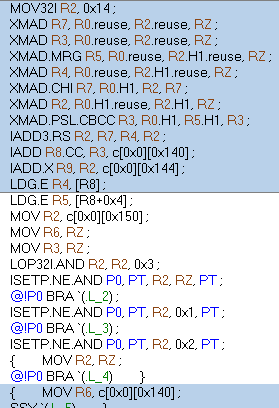
\includegraphics[width=.8\linewidth]{images/cuda_vector_type_before.png}
    \caption{Instruction for \mintinline{c}{float dist_x}}
  \end{subfigure}
  \begin{subfigure}{.5\textwidth}
    \centering
    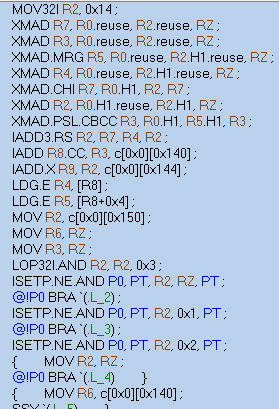
\includegraphics[width=.8\linewidth]{images/cuda_vector_type_after.png}
    \caption{Instruction for \mintinline{cuda}{float2 dist}}
  \end{subfigure}
  \caption{Instructions generated for \textbf{(a)} C++ primitive and \textbf{(b)} CUDA vector type.}
  \label{figure:cuda_vector_type}
\end{figure}

\subsection{Use CUDA Math API} \label{subsec:cuda_math_api}
The CUDA Best Practices Guide suggested that
\begin{enumerate}
  \item The reciprocal square root should always be invoked explicitly as \texttt{rsqrtf()} for
  single precision \cite{cuda_best_practices_reciprocal_sqrt}.
  \item Avoid using heavy-weight \texttt{pow()} and \texttt{powf()} functions. Use explicit
  multiplication for small integer powers \cite{cuda_best_practices_math_libraries}.
\end{enumerate}

\begin{listing}[H]
  \begin{minted}[linenos, frame=lines, framesep=2mm, fontsize=\footnotesize]{cuda}
// Before
float mag_add_soft = dist.x * dist.x + dist.y * dist.y + SOFTENING_SQUARE;
float m_div_mag = d_nbodies[j].m / (mag_add_soft * sqrtf(mag_add_soft));

// After (Version 1)
float mag_add_soft = dist.x * dist.x + dist.y * dist.y + SOFTENING_SQUARE;
float m_div_mag = d_nbodies[j].m * rsqrtf(mag_add_soft * mag_add_soft * mag_add_soft);

// After (Version 2)
float inv_dist = rsqrtf(dist.x * dist.x + dist.y * dist.y + SOFTENING_SQUARE);
float m_div_mag = d_nbodies[j].m * inv_dist * inv_dist * inv_dist;
  \end{minted}
  \caption{Converting from \texttt{sqrtf()} to \texttt{rsqrtf()}.}
  \label{listing:cuda_rsqrtf}
\end{listing}

In Assignment 1, huge performance increase was achieved by removing the usage of \texttt{powf()}
function, as shown by line 2 in \cref{listing:cuda_rsqrtf} and the formula simplification below:
\begin{equation*}
  \begin{aligned}
    (||\vec{x_j} - \vec{x_i}||^2 + \epsilon^2)^\frac{3}{2} \equiv (||\vec{x_j} - \vec{x_i}||^2 + \epsilon^2)\sqrt{(||\vec{x_j} - \vec{x_i}||^2 + \epsilon^2)} \\
  \end{aligned}
\end{equation*}

CUDA Math API provides the function \mintinline{c}{rsqrtf(float x)} that is able to calculate
\(\frac{1}{x}\) directly in the device. With this optimisation applied, the division operation can
be replaced by a multiplication operation, as demonstrated in \cref{listing:cuda_rsqrtf}.

\noindent `Version 1' represents the following equation:
\begin{equation*}
  \begin{aligned}
    (||\vec{x_j} - \vec{x_i}||^2 + \epsilon^2)^\frac{3}{2} \equiv \sqrt{(||\vec{x_j} - \vec{x_i}||^2 + \epsilon^2)^3} \\
  \end{aligned}
\end{equation*}

\noindent `Version 2' represents the following equation:
\begin{equation*}
  \begin{aligned}
    (||\vec{x_j} - \vec{x_i}||^2 + \epsilon^2)^\frac{3}{2} \equiv \left[\sqrt{(||\vec{x_j} - \vec{x_i}||^2 + \epsilon^2)}\right]^3 \\
  \end{aligned}
\end{equation*}

\renewcommand{\arraystretch}{1.3}
\begin{longtable}{|c|c|c|c|}
  \hline \endfirsthead & \multicolumn{3}{c|}{Total Execution Time (seconds)} \\ \cline{2-4}
  \multirow{-2}{*}{Value} & Before & Version 1 & Version 2 \\ \hline
  \rowcolor{lightgray}\multicolumn{4}{|c|}{\textbf{Number of Bodies (N)}} \\ \hline
  1024  & 0.078  & 0.013 & 0.011 \\
  2048  & 0.144  & 0.024 & 0.023 \\
  4096  & 0.287  & 0.057 & 0.052 \\
  10000 & 0.726  & 0.218 & 0.206 \\
  20000 & 1.859  & 0.825 & 0.769 \\
  30000 & 5.028  & 1.839 & 1.714 \\
  40000 & 7.376  & 3.246 & 3.008 \\
  50000 & 12.839 & 5.161 & 4.765 \\ \hline
  \textbf{Average speedup} & \textbf{-} & \textbf{3.76} & \textbf{4.11} \\ \hline
  \rowcolor{lightgray}\multicolumn{4}{|c|}{\textbf{Activity Grid Dimension (D)}} \\ \hline
  1000  & 0.080 & 0.019 & 0.018 \\
  2000  & 0.103 & 0.043 & 0.042 \\
  5000  & 0.267 & 0.207 & 0.206 \\
  10000 & 0.854 & 0.793 & 0.793 \\
  15000 & 1.831 & 1.770 & 1.770 \\ \hline
  \textbf{Average speedup} & \textbf{-} & \textbf{2.00} & \textbf{2.06} \\ \hline
  \caption{Performance comparison of different number of threads per block.}
  \label{table:cuda_rsqrtf}
\end{longtable}
\renewcommand{\arraystretch}{1}

As shown in \cref{table:cuda_rsqrtf}, great performance speedup is achieved by using the CUDA Math
API. Although both `Version 1' and `Version 2' represent a different variant of the same equation,
`Version 2' provides a higher performance speedup than `Version 1'.

However, one disadvantage is that \texttt{rsqrtf()} has a maximum ULP (Unit of Least Precision)
error of 2 \cite{math_standard_func}. This error is acceptable as the actual difference would be
small, and it has also provided a significant amount of performance improvements.

\subsection{Summary}
\begin{figure}[H]
  \centering
  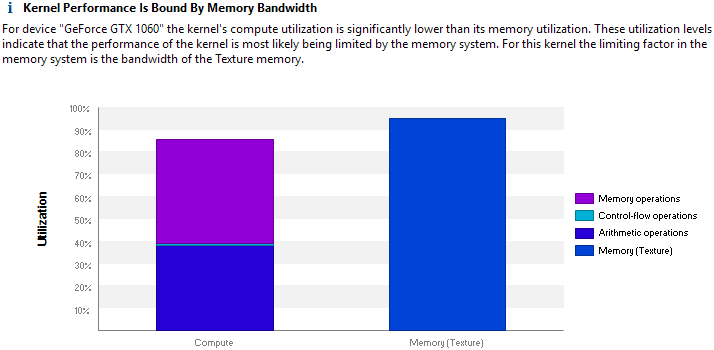
\includegraphics[width=\textwidth]{images/rsqrtf_kernel_analysis_compute_force.png}
  \caption{Kernel analysis of \texttt{compute\_force} after \texttt{rsqrtf()}.}
  \label{figure:rsqrtf_kernel_analysis_compute_force}
\end{figure}

\begin{enumerate}
  \item Comparing \cref{figure:rsqrtf_kernel_analysis_compute_force} with
  \cref{figure:baseline_kernel_analysis_compute_force}, both compute and memory utilisation have
  increased significantly after using CUDA's \texttt{rsqrtf()} to calculate the reciprocal square
  root.
  \item The kernel performance of \texttt{compute\_force} is now limited by the memory bandwidth.
\end{enumerate}

% ======================================================
\pagebreak
\section{Improving Memory Bandwidth}
\subsection{Store Runtime Constants into Constant Memory}
The runtime constants are currently passed to the kernel function as arguments.

\begin{listing}[H]
  \begin{minted}[linenos, frame=lines, framesep=2mm, fontsize=\footnotesize]{cuda}
// Before
__global__ void update_body(const unsigned int N,
                            const unsigned int D,
                            const unsigned int grid_size, ...)
...
__global__ void normalise_activity_map(const unsigned int grid_size,
                                       const float normalising_factor, ...)
// After
__constant__ unsigned int c_N;
__constant__ unsigned int c_D;
__constant__ unsigned int c_grid_size;
__constant__ float c_normalising_factor;
...
__global__ void parallelise_each_body(nbody *d_nbodies, float *d_activity_map)
__global__ void normalise_activity_map(float *d_activity_map)
  \end{minted}
  \caption{Store runtime constants into constant memory.}
  \label{listing:constant_runtime_constants}
\end{listing}

\renewcommand{\arraystretch}{1.3}
\begin{longtable}{|c|c|c|c|}
  \hline \endfirsthead & \multicolumn{2}{c|}{Total Execution Time (seconds)} & \\ \cline{2-3}
  \multirow{-2}{*}{Value} & Before & After & \multirow{-2}{*}{Speedup} \\ \hline
  \rowcolor{lightgray}\multicolumn{4}{|c|}{\textbf{Number of Bodies (N)}} \\ \hline
  1024  & 0.011 & 0.012 & 0.92 \\
  2048  & 0.022 & 0.024 & 0.92 \\
  4096  & 0.052 & 0.051 & 1.02 \\
  10000 & 0.205 & 0.201 & 1.02 \\
  20000 & 0.768 & 0.764 & 1.01 \\
  30000 & 1.718 & 1.693 & 1.01 \\
  40000 & 3.006 & 2.996 & 1.00 \\
  50000 & 4.763 & 4.712 & 1.01 \\ \hline
  \multicolumn{3}{|r|}{\textbf{Average}} & \textbf{0.99} \\ \hline
  \rowcolor{lightgray}\multicolumn{4}{|c|}{\textbf{Activity Grid Dimension (D)}} \\ \hline
  1000  & 0.018 & 0.019 & 0.95 \\
  2000  & 0.042 & 0.043 & 0.98 \\
  5000  & 0.206 & 0.207 & 1.00 \\
  10000 & 0.793 & 0.793 & 1.00 \\
  15000 & 1.770 & 1.771 & 1.00 \\ \hline
  \multicolumn{3}{|r|}{\textbf{Average}} & \textbf{0.98} \\ \hline
  \caption{Performance speedup of loading runtime constants from constant memory.}
  \label{table:constant_runtime_constants}
\end{longtable}
\renewcommand{\arraystretch}{1}

The results in \cref{table:constant_runtime_constants} have shown that loading the constants from
constant memory is slightly slower than passing them as arguments for small number of \textbf{N}
(\(\lessapprox 4096\)). When \textbf{N} is \(\gtrapprox 10000\), there is a noticeable reduction in
the total execution time.

According to the CUDA Programming Guide, \mintinline{cuda}{__global__} function parameters are
passed to the device via constant memory \cite{func_params}. However, as demonstrated by
\cref{listing:compare_runtime_constant} and \cref{figure:compare_runtime_constant}, the variable is
stored in a different constant memory location when it is used differently.

\begin{listing}[H]
  \begin{minted}[linenos, frame=lines, framesep=2mm, fontsize=\footnotesize]{cuda}
__constant__ float c_grid_size;

__global__ normalise_activity_map(const float grid_size) {
    const unsigned int i = blockIdx.x * blockDim.x + threadIdx.x;

    if (i < grid_size)   // Figure 8(a)
    if (i < c_grid_size) // Figure 8(b)
}
  \end{minted}
  \caption{Implementation comparison for accessing the runtime constant.}
  \label{listing:compare_runtime_constant}
\end{listing}

\begin{figure}[ht]
  \begin{subfigure}{.5\textwidth}
    \centering
    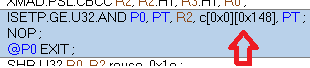
\includegraphics[width=.9\linewidth]{images/constant_memory_before.png}
    \caption{\mintinline{cuda}{__global__} function parameter.}
  \end{subfigure}
  \begin{subfigure}{.5\textwidth}
    \centering
    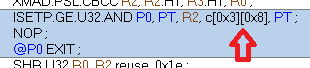
\includegraphics[width=.9\linewidth]{images/constant_memory_after.png}
    \caption{\mintinline{cuda}{__constant__} qualifier variable.}
  \end{subfigure}
  \caption{Constant memory location of different implementation.}
  \label{figure:compare_runtime_constant}
\end{figure}

\subsection{Global Memory Alignment and Access Pattern}
\begin{figure}[H]
  \centering
  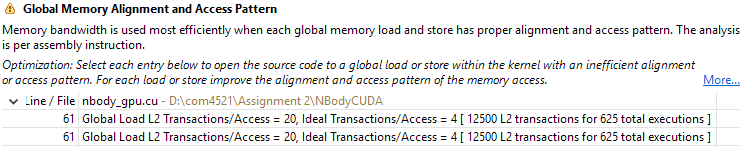
\includegraphics[width=\textwidth]{images/baseline_global_access_pattern.png}
  \caption{Ineffective global memory access in \texttt{compute\_force}.}
  \label{figure:baseline_memory_bandwidth_analysis}
\end{figure}

\begin{listing}[ht]
  \begin{minted}[linenos, firstnumber=61, frame=lines, framesep=2mm, fontsize=\footnotesize]{cuda}
float2 dist = make_float2(d_nbodies[j].x - d_nbodies[i].x, d_nbodies[j].y - d_nbodies[i].y);
  \end{minted}
  \caption{Strided access of 5 for \texttt{d\_nbodies} members, 20\% bandwidth only.}
\end{listing}

As shown in \cref{figure:baseline_memory_bandwidth_analysis}, the kernel \texttt{compute\_force} is
performing 5 times more transactions per access than ideal. This issue can be solved by changing the
layout of \texttt{d\_nbodies} from AoS to SoA. Three possible implementations are considered and
documented in \cref{subsubsec:soa_struct_by_value}, \cref{subsubsec:soa_struct_member}, and
\cref{subsubsec:soa_struct_by_reference}.

\subsubsection{Passing SoA \texorpdfstring{\mintinline{c}{struct}}{} by Value (Version 1)} \label{subsubsec:soa_struct_by_value}
\begin{listing}[H]
  \begin{minted}[linenos, frame=lines, framesep=2mm, fontsize=\footnotesize]{cuda}
nbody_soa d_nbodies;
...
/* Memory cost = the size of a nbody_soa structure (40 bytes) */
compute_force<<<blocks, threads>>>(d_nbodies, ...);
...
__global__ void compute_force(nbody_soa d_nbodies, ...)
  \end{minted}
  \caption{Passing \mintinline{c}{struct nbody_soa} to \texttt{compute\_force} by value.}
\end{listing}

\subsubsection{Passing SoA \texorpdfstring{\mintinline{c}{struct}}{} Members by Reference (Version 2)} \label{subsubsec:soa_struct_member}
\begin{listing}[H]
  \begin{minted}[linenos, frame=lines, framesep=2mm, fontsize=\footnotesize]{cuda}
nbody_soa d_nbodies;
...
/* Memory cost = 3 pointers (3 * 8 bytes = 24 bytes) */
compute_force<<<blocks, threads>>>(d_nbodies.x, d_nbodies.y,  d_nbodies.m, ...);
...
__global__ void compute_force(float *x, float *y, float *m, ...)
  \end{minted}
  \caption{Passing the \texttt{x}, \texttt{y}, and \texttt{m} to \texttt{compute\_force} by reference.}
\end{listing}

\subsubsection{Passing SoA \texorpdfstring{\mintinline{c}{struct}}{} by Reference (Version 3)} \label{subsubsec:soa_struct_by_reference}

\begin{listing}[H]
  \begin{minted}[linenos, frame=lines, framesep=2mm, fontsize=\footnotesize]{cuda}
nbody_soa h_nbodies, *d_nbodies;
float *d_x, *d_y, *d_vx, *d_vy, *d_m; // Individual pointers to device memory

// Allocate device memory
checkCudaError(cudaMalloc((void **)(&d_nbodies), sizeof(nbody_soa)));
checkCudaError(cudaMalloc((void **)(&d_x), nbodies_soa_size));
...
// Copy host data to individual pointers first
checkCudaError(cudaMemcpy(d_x, h_nbodies.x, nbodies_soa_size, cudaMemcpyHostToDevice));
...
// Copy individual pointers to SoA pointer
checkCudaError(cudaMemcpy(d_nbodies, &h_nbodies, sizeof(nbody_soa), cudaMemcpyHostToDevice));
checkCudaError(cudaMemcpy(&d_nbodies->x, &d_x, sizeof(float *), cudaMemcpyHostToDevice));
...
/* Memory cost = 1 pointer (8 bytes) */
compute_force<<<blocks, threads>>>(d_nbodies, ...);
...
__global__ void compute_force(nbody_soa *d_nbodies, ...)
  \end{minted}
  \caption{Passing \mintinline{c}{struct nbody_soa} by reference.}
  \label{listing:soa_version_3}
\end{listing}

As shown in \cref{listing:soa_version_3}, Version 3 has a more complex implementation than Version 1
and 2. This is because calling \mintinline{cuda}{cudaMalloc()} directly on \texttt{d\_nbodies->x}
will raise an `Access violation writing location' at runtime. Therefore, it is required to allocate
device memory to those individual device pointers first, then copy them to the SoA pointer members.

\subsubsection{Results and Summary}
After changing the data layout of \texttt{d\_nbodies} to Structure of Arrays, Visual Profiler no
longer shows the access pattern warning. However, \cref{table:soa_layout} shows that the performance
of SoA is slightly slower than AoS.
\renewcommand{\arraystretch}{1.3}
\begin{longtable}{|c|c|c|c|c|}
  \hline \endfirsthead & \multicolumn{4}{c|}{Total Execution Time (seconds)} \\ \cline{2-5}
  \multirow{-2}{*}{Value} & Before (AoS) & Version 1 & Version 2 & Version 3 \\ \hline
  \rowcolor{lightgray}\multicolumn{5}{|c|}{\textbf{Number of Bodies (N)}} \\ \hline
  1024  & 0.012 & 0.011 & 0.011 & 0.012 \\
  2048  & 0.024 & 0.021 & 0.021 & 0.022 \\
  4096  & 0.051 & 0.052 & 0.052 & 0.052 \\
  10000 & 0.202 & 0.227 & 0.227 & 0.233 \\
  20000 & 0.763 & 0.824 & 0.824 & 0.783 \\
  30000 & 1.695 & 2.030 & 2.028 & 1.857 \\
  40000 & 2.996 & 3.076 & 3.075 & 3.045 \\
  50000 & 4.707 & 4.754 & 4.751 & 4.869 \\ \hline
  \textbf{Average speedup} & \textbf{-} & \textbf{0.98} & \textbf{0.98} & \textbf{0.97} \\ \hline
  \rowcolor{lightgray}\multicolumn{5}{|c|}{\textbf{Activity Grid Dimension (D)}} \\ \hline
  1000  & 0.019 & 0.020 & 0.020 & 0.020 \\
  2000  & 0.043 & 0.043 & 0.043 & 0.044 \\
  5000  & 0.207 & 0.207 & 0.207 & 0.208 \\
  10000 & 0.793 & 0.794 & 0.794 & 0.794 \\
  15000 & 1.770 & 1.772 & 1.771 & 1.771 \\ \hline
  \textbf{Average speedup} & \textbf{-} & \textbf{0.99} & \textbf{0.99} & \textbf{0.98} \\ \hline
  \caption{Performance comparison of different SoA implementations.}
  \label{table:soa_layout}
\end{longtable}
\renewcommand{\arraystretch}{1}

\begin{figure}[ht]
  \centering
  \begin{subfigure}{\textwidth}
    \centering
    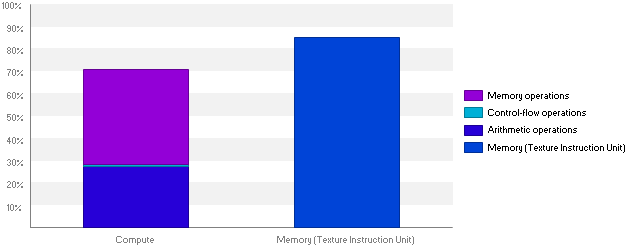
\includegraphics[width=\textwidth]{images/soa_v1_global_mem.png}
    \caption{SoA Version 1, texture memory}
  \end{subfigure}
\end{figure}
\begin{figure}[ht]\ContinuedFloat
  \centering
  \begin{subfigure}{.95\textwidth}
    \centering
    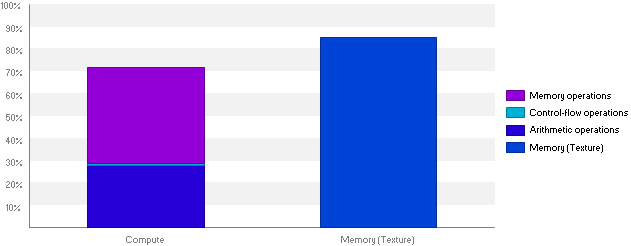
\includegraphics[width=\textwidth]{images/soa_v2_global_mem.png}
    \caption{SoA Version 2, texture memory}
    \label{figure:soa_v2_global_mem}
  \end{subfigure}\\ \bigskip
  \begin{subfigure}{.95\textwidth}
    \centering
    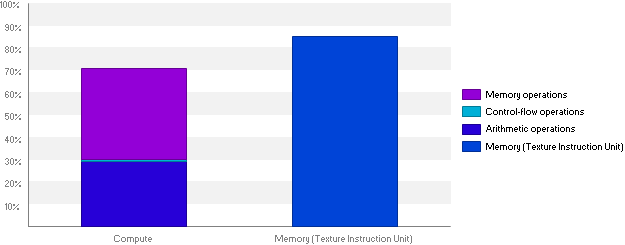
\includegraphics[width=\textwidth]{images/soa_v3_global_mem.png}
    \caption{SoA Version 3, texture memory}
  \end{subfigure}
  \caption{Kernel analysis of \texttt{compute\_force} on 3 different SoA implementations.}
  \label{figure:soa_layout}
\end{figure}

As illustrated by \cref{figure:soa_layout}, both compute and memory utilisation have decreased after
changing from AoS to SoA (in comparison with \cref{figure:rsqrtf_kernel_analysis_compute_force}).
This explains why the three versions of the SoA implementation has longer execution time than AoS.

In terms of compute utilisation, SoA Version 2 is the highest among the three versions (\(\approx
71\%\)). All three implementations are limited by the bandwidth of texture memory.

\subsection{Read-Only Memory for SoA}
Since SoA Version 2 (\cref{subsubsec:soa_struct_member}) and Version 3
\cref{subsubsec:soa_struct_by_reference} are passing the pointers, they can be further optimised by
using read-only memory.

\begin{listing}[H]
  \begin{minted}[linenos, frame=lines, framesep=2mm, fontsize=\footnotesize]{cuda}
// SoA Version 2
__global__ void compute_force(float const *__restrict__  x,
                              float const *__restrict__  y,
                              float const *__restrict__  m, ...)
// SoA Version 3
__global__ void compute_force(nbody_soa const *__restrict__  d_nbodies, ...)
  \end{minted}
  \caption{Adding \mintinline{cuda}{__restrict__} specifier to SoA pointers.}
\end{listing}

\subsubsection{Results and Summary}
\renewcommand{\arraystretch}{1.3}
\begin{longtable}{|c|c||c|c||c|c|}
  \hline \endfirsthead & \multicolumn{5}{c|}{Total Execution Time (seconds)} \\ \cline{2-6}
  \multirow{-2}{*}{Value} & AoS (baseline) & V2 (tex.) & V2 (read) & V3 (tex.) & V3 (read) \\ \hline
  \rowcolor{lightgray}\multicolumn{6}{|c|}{\textbf{Number of Bodies (N)}} \\ \hline
  1024  & 0.012 & 0.011 & 0.012 & 0.012 & 0.012 \\
  2048  & 0.024 & 0.021 & 0.017 & 0.022 & 0.022 \\
  4096  & 0.051 & 0.052 & 0.044 & 0.052 & 0.052 \\
  10000 & 0.202 & 0.227 & 0.187 & 0.233 & 0.229 \\
  20000 & 0.763 & 0.824 & 0.744 & 0.783 & 0.774 \\
  30000 & 1.695 & 2.028 & 1.667 & 1.857 & 1.835 \\
  40000 & 2.996 & 3.075 & 2.970 & 3.045 & 3.009 \\
  50000 & 4.707 & 4.751 & 4.655 & 4.869 & 4.826 \\ \hline
  \textbf{Average speedup} & \textbf{-} & \textbf{0.98} & \textbf{1.09} & \textbf{0.97} &
  \textbf{0.98} \\ \hline
  \rowcolor{lightgray}\multicolumn{6}{|c|}{\textbf{Activity Grid Dimension (D)}} \\ \hline
  1000  & 0.019 & 0.020 & 0.018 & 0.020 & 0.020 \\
  2000  & 0.043 & 0.043 & 0.042 & 0.044 & 0.044 \\
  5000  & 0.207 & 0.207 & 0.206 & 0.208 & 0.208 \\
  10000 & 0.793 & 0.794 & 0.792 & 0.794 & 0.794 \\
  15000 & 1.770 & 1.771 & 1.769 & 1.771 & 1.771 \\ \hline
  \textbf{Average speedup} & \textbf{-} & \textbf{0.99} & \textbf{1.02} & \textbf{0.98} &
  \textbf{0.98} \\ \hline
  \caption{Performance comparison between SoA texture memory and read-only memory.}
  \label{table:soa_read_only_mem}
\end{longtable}
\renewcommand{\arraystretch}{1}

As shown in \cref{table:soa_read_only_mem}, read-only memory is faster than texture memory. In
particular, SoA Version 2 with read-only memory provides a minor performance improvement. Moreover,
both compute and memory utlisation of SoA Version 2 has increased when compared to texture memory
(\cref{figure:soa_v2_global_mem}).

\noindent \textbf{Conclusion:} SoA Version 2 is selected as it has the best performance up to this
point.

\begin{figure}[ht]
  \centering
  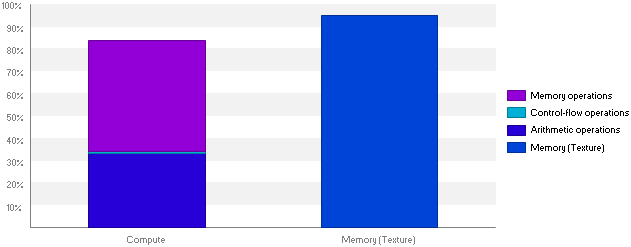
\includegraphics[width=.82\textwidth]{images/soa_v2_read_only_mem.png}
  \caption{Kernel analysis of \texttt{compute\_force} with SoA Version 2, read-only memory.}
  \label{figure:soa_v2_read_only_mem}
\end{figure}

\subsubsection{Optimise for Pointer Aliasing} \label{subsubsec:optimise_pointer_aliasing}
According to a CUDA blog post \cite{cuda_blog_pointer_aliasing} and the CUDA Programming Guide for
\cite{restrict}, it is suggested to use the \mintinline{cuda}{__restrict__} keyword on pointers if
it is known that the pointers will not be used to access overlapping regions. This tells the
compiler that these pointers are not aliased, and the compiler can now perform some low-level
optimisations.

\cref{listing:optimise_pointer_aliasing} is considered an optimisation ahead. No observable
improvements are recorded as both \texttt{update\_body} and \texttt{normalise\_activity\_map} have
the lowest optimisation priority (\cref{figure:baseline_kernel_optimisation_priority}).

\begin{listing}[H]
  \begin{minted}[linenos, frame=lines, framesep=2mm, fontsize=\footnotesize]{cuda}
/* Kernel: update_body */
// Before
__global__ void update_body(nbody_soa d_nbodies)

// After
__global__ void update_body(float *__restrict__ x,
                            float *__restrict__ y,
                            float *__restrict__ vx,
                            float *__restrict__ vy, ...)

/* Kernel: normalise_activity_map */
// Before
__global__ void normalise_activity_map(float *d_activity_map) {

// After
__global__ void normalise_activity_map(float *__restrict__ d_activity_map) {
  \end{minted}
  \caption{Adding \mintinline{cuda}{__restrict__} specifier to SoA pointers.}
  \label{listing:optimise_pointer_aliasing}
\end{listing}

% ======================================================
\subsection{Shared Memory}
\subsubsection{Problem: Conditional Synchronisation, N-Bodies Out of Sync}
\begin{listing}[H]
  \begin{minted}[linenos, frame=lines, framesep=2mm, fontsize=\footnotesize]{cuda}
__global__ void compute_force(...) {
    const unsigned int i = blockIdx.x * blockDim.x + threadIdx.x;
    __shared__ float3 s_nbodies[THREADS_PER_BLOCK];

    // Conditional __syncthreads() (bad)
    if (i < N) {
        for (unsigned int sub_block = 0; sub_block < gridDim.x; ++sub_block) {
            s_nbodies[threadIdx.x] = ...
            __syncthreads();

            for (unsigned int j = 0; j < THREADS_PER_BLOCK; ++j) { ... }
            __syncthreads();
        }
        ...
    }
}
  \end{minted}
  \caption{\texttt{if} statement (line 6) preventing \texttt{\_\_syncthreads()} from functioning correctly.}
  \label{listing:shared_mem_difficulty}
\end{listing}

\begin{figure}[H]
  \centering
  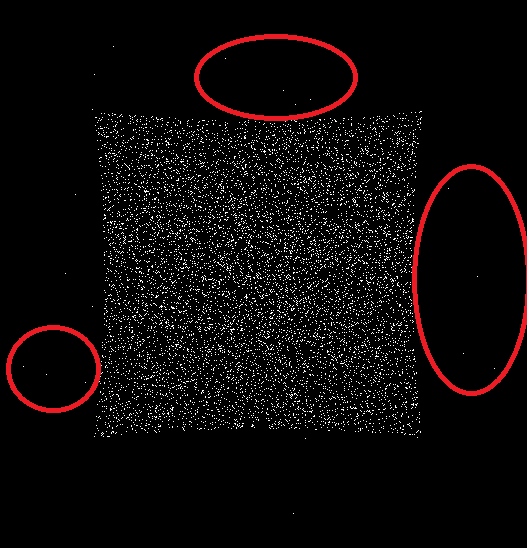
\includegraphics[width=\textwidth]{images/shared_mem_difficulty.png}
  \caption{Some n-bodies (red circles) are out of sync.}
  \label{figure:shared_mem_difficulty}
\end{figure}

As demonstrated in \cref{figure:shared_mem_difficulty}, some n-bodies converge slower than the group
of n-bodies. This problem does not exist when the number of bodies (\textbf{N}) is a multiple of
\texttt{THREADS\_PER\_BLOCK}. When \textbf{N} is not a multiple of \texttt{THREADS\_PER\_BLOCK},
then there will be \texttt{N \% THREADS\_PER\_BLOCK} n-bodies out of sync. For example:
\begin{itemize}
  \item $\textbf{N} =$ 10240, 256 threads per block: No n-bodies out of sync.
  \item $\textbf{N} =$ 10270, 256 threads per block: 30 n-bodies out of sync.
\end{itemize}

\textbf{Cause:} According to the CUDA Programming Guide \cite{sync_functions},
\texttt{\_\_syncthreads()} is allowed in conditional code but only if the conditional evaluates
identically across the entire thread block, otherwise the code execution is likely to hang or
produce unintended side effects.

\subsubsection{Solution}
\begin{listing}[H]
  \begin{minted}[linenos, frame=lines, framesep=2mm, fontsize=\footnotesize]{cuda}
__global__ void compute_force(float const *__restrict__ x, ...) {
    __shared__ float3 s_nbodies[THREADS_PER_BLOCK];
    const unsigned int i = blockIdx.x * blockDim.x + threadIdx.x;

    for (unsigned int sub_block = 0; sub_block < gridDim.x; ++sub_block) {
        // Inline conditional below to prevent reading beyond allocated
        s_nbodies[threadIdx.x] = sub_i < c_N
                                    ? make_float3(x[sub_i], ...)
                                    : make_float3(0, 0, 0);
        __syncthreads();

        // Do not compute force for non-existent n-body
        if (i < c_N) {
            for (unsigned int j = 0; j < THREADS_PER_BLOCK; ++j) { ... }
        }

        __syncthreads();
    }
}
  \end{minted}
  \caption{Solution for the problem in \cref{figure:shared_mem_difficulty}.}
  \label{listing:shared_mem_solution}
\end{listing}

The problem can be solved by moving the conditional inside the loop, as shown in
\cref{listing:shared_mem_solution}. By doing this, all threads are guaranteed to reach the
\texttt{\_\_syncthreads()}. However, this will introduced an additional conditional branch inside
the loop to prevent reading beyond allocated (line 7).

\subsubsection{Results} \label{subsec:shared_mem_results}
\renewcommand{\arraystretch}{1.3}
\begin{longtable}{|c|c|c|c|}
  \hline \endfirsthead & \multicolumn{3}{c|}{Total Execution Time (seconds)} \\ \cline{2-4}
  \multirow{-2}{*}{Value} & Before (\cref{subsubsec:optimise_pointer_aliasing} version) & After &
  Speedup \\ \hline
  \rowcolor{lightgray}\multicolumn{4}{|c|}{\textbf{Number of Bodies (N)}} \\ \hline
  1024  & 0.011 & 0.005 & 2.20 \\
  2048  & 0.018 & 0.009 & 2.00 \\
  4096  & 0.044 & 0.022 & 2.00 \\
  10000 & 0.187 & 0.093 & 2.01 \\
  20000 & 0.744 & 0.361 & 2.06 \\
  30000 & 1.667 & 0.846 & 1.97 \\
  40000 & 2.968 & 1.426 & 2.08 \\
  50000 & 4.658 & 2.269 & 2.05 \\ \hline
  \multicolumn{3}{|r|}{\textbf{Average}} & \textbf{2.05} \\ \hline
  \rowcolor{lightgray}\multicolumn{4}{|c|}{\textbf{Activity Grid Dimension (D)}} \\ \hline
  100   & 0.018 & 0.012 & 1.50 \\
  1000  & 0.042 & 0.036 & 1.17 \\
  2000  & 0.206 & 0.200 & 1.03 \\
  5000  & 0.792 & 0.787 & 1.01 \\
  10000 & 1.769 & 1.763 & 1.00 \\ \hline
  \multicolumn{3}{|r|}{\textbf{Average}} & \textbf{1.14} \\ \hline
  \caption{Performance speedup of using shared memory for n-bodies array.}
  \label{table:shared_mem_soa}
\end{longtable}
\renewcommand{\arraystretch}{1}

As shown in \cref{table:shared_mem_soa}, the performance for various values of \textbf{N} is 2 times
faster when using shared memory. For \textbf{D}, the performance speedup decreases as \textbf{D}
increases.

\subsubsection{Summary}

\begin{figure}[ht]
  \centering
  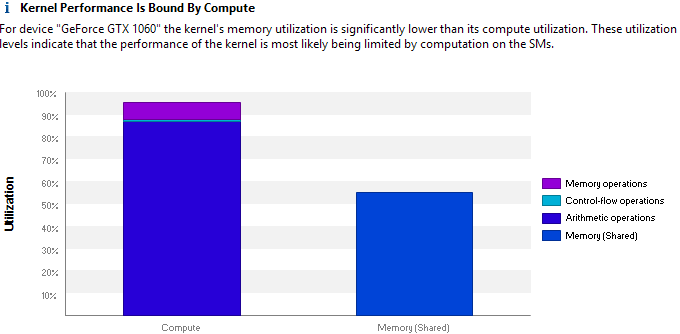
\includegraphics[width=\textwidth]{images/shared_mem_kernel_analysis_compute_force.png}
  \caption{Kernel analysis of \texttt{compute\_force} after using shared memory.}
  \label{figure:shared_mem_kernel_analysis_compute_force}
\end{figure}

\begin{figure}[ht]
  \begin{subfigure}{\textwidth}
    \centering
    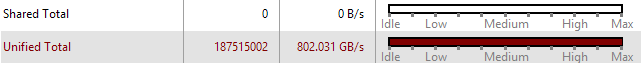
\includegraphics[width=\textwidth]{images/bandwidth_before_shared_mem.png}
    \caption{Before using shared memory}
  \end{subfigure}
\end{figure}
\begin{figure}[ht] \ContinuedFloat
  \begin{subfigure}{\textwidth}
    \centering
    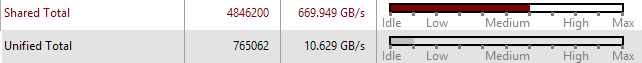
\includegraphics[width=\textwidth]{images/bandwidth_after_shared_mem.png}
    \caption{After using shared memory}
  \end{subfigure}
\end{figure}

\begin{enumerate}
  \item According to \cref{figure:shared_mem_kernel_analysis_compute_force}, memory operations have
  reduced significantly and the kernel performance is now limited by arithmetic operations.
  \item Global memory loads are reduced by using shared memory to cache the n-bodies.
\end{enumerate}

\pagebreak
\subsection{Dynamically Calculate Shared Memory Usage}
Currently the shared memory is using 256 threads per block (inherited from baseline implementation).
\cref{listing:dynamic_shared_mem} attempts to improve the performance by using the optimal block
size calculated by CUDA API.

\begin{listing}[H]
  \begin{minted}[linenos, frame=lines, framesep=2mm, fontsize=\footnotesize]{cuda}
int requiredSM(int blockSize) {
    return blockSize * sizeof(float3);
}
...
cudaOccupancyMaxPotentialBlockSizeVariableSMem(&minGridSize, &block_size,
                                               compute_force, requiredSM);
...
compute_force<<<blocksPerGrid, block_size, requiredSM(block_size)>>>(...);
  \end{minted}
  \caption{Calculating block size that achieves maximum potential occupancy.}
  \label{listing:dynamic_shared_mem}
\end{listing}

\renewcommand{\arraystretch}{1.3}
\begin{longtable}{|c|c|c|c|}
  \hline \endfirsthead & \multicolumn{2}{c|}{Total Execution Time (seconds)} & \\ \cline{2-3}
  \multirow{-2}{*}{Value} & Before (Static shared, 256 block size) & After (Dynamic) &
  \multirow{-2}{*}{Speedup} \\ \hline
  \rowcolor{lightgray}\multicolumn{4}{|c|}{\textbf{Number of Bodies (N)}} \\ \hline
  1024  & 0.005 & 0.014 & 0.36 \\
  2048  & 0.009 & 0.023 & 0.39 \\
  4096  & 0.022 & 0.045 & 0.49 \\
  10000 & 0.093 & 0.113 & 0.82 \\
  20000 & 0.360 & 0.446 & 0.81 \\
  30000 & 0.850 & 1.002 & 0.85 \\
  40000 & 1.425 & 1.781 & 0.80 \\
  50000 & 2.270 & 2.728 & 0.83 \\ \hline
  \multicolumn{3}{|r|}{\textbf{Average}} & \textbf{0.67} \\ \hline
  \rowcolor{lightgray}\multicolumn{4}{|c|}{\textbf{Activity Grid Dimension (D)}} \\ \hline
  100   & 0.012 & 0.019 & 0.63 \\
  1000  & 0.036 & 0.043 & 0.84 \\
  2000  & 0.200 & 0.207 & 0.97 \\
  5000  & 0.786 & 0.794 & 0.99 \\
  10000 & 1.763 & 1.770 & 1.00 \\ \hline
  \multicolumn{3}{|r|}{\textbf{Average}} & \textbf{0.88} \\ \hline
  \caption{Performance comparison of static and dynamic size for shared memory.}
  \label{table:dynamic_shared_mem}
\end{longtable}
\renewcommand{\arraystretch}{1}

\textbf{Summary:} Using the block size calculated by CUDA produces worse performance. CUDA returned
a block size of 1024, which causes the larger performance loss when the value of \textbf{N} is
smaller. This has led to inefficient execution as the `tail' of the blocks are large. Therefore, it
is not suitable to use this technique.

% ======================================================
\pagebreak
\section{Compute Analysis}
\subsection{Limitations}
\begin{figure}[ht]
  \centering
  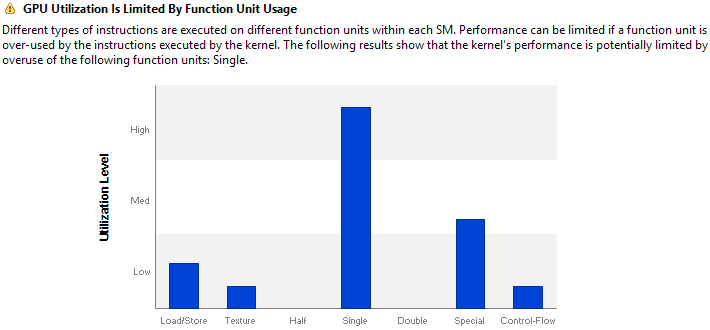
\includegraphics[width=\textwidth]{images/compute_analysis_shared_mem_compute_force.png}
  \caption{Single precision instructions limiting kernel performance.}
  \label{figure:compute_analysis_shared_mem_compute_force}
\end{figure}

\begin{listing}[H]
  \begin{minted}[linenos, frame=lines, framesep=2mm, fontsize=\footnotesize]{cuda}
const float2 dist = make_float2(s_nbody.x - x[i], s_nbody.y - y[i]);
const float inv_dist = rsqrtf(dist.x * dist.x + dist.y * dist.y + SOFTENING_SQUARE);
const float m_div_mag = s_nbody.z * inv_dist * inv_dist * inv_dist;

// Execution dependency, line 6, 7 depends on line 1, 3
local_sum.x += m_div_mag * dist.x;
local_sum.y += m_div_mag * dist.y;
  \end{minted}
  \caption{Most compute intensive part of the \texttt{compute\_force} kernel.}
  \label{listing:compute_analysis}
\end{listing}

As shown in \cref{figure:compute_analysis_shared_mem_compute_force}, the only limiting factor is the
single precision instructions. Special instructions are unavoidable as the equation requires square
root calculation. Some conditional statements are also required to prevent reading beyond allocated
when \textbf{N} is not a multiple of block size.

There is also an unavoidable execution dependency in \cref{listing:compute_analysis}. This increases
the latency of \texttt{compute\_force} kernel as warps would be stalling waiting for the previous
instructions to complete.

\subsection{Possible Improvements}
\noindent \textbf{Question:} Is it possible to speed up the single precision computation?

In terms of code optimisation, the possibility is low. A significant improvement was already
achieved by using CUDA \texttt{rsqrtf()} function in \cref{subsec:cuda_math_api}, and the
calculations are all in its simplest form. Running the simulation on a better GPU with higher
processing power (GFLOPS) might be the easiest way. \\[8pt]


\noindent \textbf{Question:} Is it possible to reduce the amount of computation of the current
implementation?

The answer is yes. The current implementation is calculating the summation of force \(n^2\) times.
In \cref{equation:force}, it is required to calculate the term \(\frac{(\vec{x_j} -
\vec{x_i})}{(||\vec{x_j} - \vec{x_i}||^2 + \epsilon^2)^\frac{3}{2}}\) \(n\) times for each body.

\begin{equation}
  \vec{F_i} = Gm_i \sum_{j=1}^{N} \frac{m_j(\vec{x_j} - \vec{x_i})}{(||\vec{x_j} - \vec{x_i}||^2 + \epsilon^2)^\frac{3}{2}}
  \label{equation:force}
\end{equation}

However, it is known that
\begin{align}
\vec{x_j} - \vec{x_i}       &\equiv -(\vec{x_i} - \vec{x_j}) \\
\nonumber \\
||\vec{x_j} - \vec{x_i}||^2 &\equiv ||\vec{x_i} - \vec{x_j}||^2
\end{align}

Let matrix \(D\), where \(d_{ij} = \vec{x_j} - \vec{x_i}\) initially represents the distance between
\(i^{th}\) and \(j^{th}\) body,
\[
D = \begin{bmatrix}
    d_{11} & \dots  & d_{1n} \\
    \vdots & \ddots & \vdots \\
    d_{n1} & \dots  & d_{nn}
    \end{bmatrix}
\]

Substituting (2) into matrix \(D\),
\begin{align}
D = \begin{bmatrix}
    0       & d_{12}  & d_{13}  & \dots  & d_{1n} \\
    -d_{12} & 0       & d_{23}  & \dots  & d_{2n} \\
    -d_{13} & -d_{23} & 0       & \dots  & d_{3n} \\
    \vdots  & \vdots  & \vdots  & \ddots & \vdots \\
    -d_{1n} & -d_{2n} & -d_{3n} & \dots  & 0
    \end{bmatrix}
\end{align}

As seen in (4), \(D\) is now similar to a symmetric matrix except that the elements in lower
triangular are the opposite of the one in upper triangular.

According to (3), the term \((||\vec{x_j} - \vec{x_i}||^2 + \epsilon^2)^\frac{3}{2}\) can therefore
be applied into matrix \(D\) as well,
\begin{align}
D = \begin{bmatrix}
    0       & \frac{d_{12}}{(||d_{12}||^2 + \epsilon^2)^\frac{3}{2}} & \dots  & \dots  & \frac{d_{1n}}{(||d_{1n}||^2 + \epsilon^2)^\frac{3}{2}} \\
    \frac{-d_{12}}{(||d_{12}||^2 + \epsilon^2)^\frac{3}{2}}          & 0      & \dots  & \dots  & \frac{d_{2n}}{(||d_{2n}||^2 + \epsilon^2)^\frac{3}{2}} \\
    \vdots  & \vdots  & \vdots & \ddots & \vdots \\
    \frac{-d_{1n}}{(||d_{1n}||^2 + \epsilon^2)^\frac{3}{2}} & \frac{-d_{2n}}{(||d_{2n}||^2 + \epsilon^2)^\frac{3}{2}} & \dots  & \dots  & 0
    \end{bmatrix}
\end{align}

As shown in (5), it is only required either the upper triangular or lower triangular of the matrix.
Since each body could have different mass, it cannot be integrated into matrix \(D\).

Assuming the size of the matrix is \(N\),
\begin{align*}
  \text{Total elements in upper triangular} &= \frac{N(N - 1)}{2} \\
  \text{Total elements in the matrix}       &= N^2 \\
  \\
  \therefore N^2 - \frac{N(N - 1)}{2} &= \frac{N(N + 1)}{2} \quad \text{less computations to do}
\end{align*}

\subsection{Feasibility of the Matrix Implementation} \label{subsec:triangular_matrix}
A potential \(\mathcal{O}(n^2)\) performance improvement is good, but the implementation difficulty
might have exceeded the scope of this assignment.

Below is a preliminary analysis of the matrix implementation procedure:
\begin{enumerate}
  \item Allocate a triangular array of size \mintinline{cuda}{sizeof(float2) * N * (N - 1) / 2}.
  Vector type is required to represent the distance with \texttt{x} and \texttt{y}.
  \item Define a new kernel that is responsible for calculating the upper (or lower) triangular
  \item For simplicity, launch the kernel with 1D block size.
  \item Since the upper triangular is now represented by an 1D array, it will need special equations
  to calculate the corresponding \((row, column)\) for a given linear index. Navarro and Hitschfeld
  \cite{navarro_2014} has provided an equation in that uses block-wise mapping to calculate the
  \((row, column)\).
  \item For each linear index, calculate the \((row, column)\).
  \item Compute \(\cfrac{(\vec{x_{col}} - \vec{x_{row}})}{(||\vec{x_{col}} - \vec{x_{row}}||^2 +
  \epsilon^2)^\frac{3}{2}}\)
  \item Store the result into the array.
\end{enumerate}
\bigskip
\noindent There are several challenges that must be overcome:
\begin{enumerate}
  \item \textbf{Memory Access Pattern:} In this implementation, each thread of a warp are not
  accessing the adjacent \texttt{x} and \texttt{y}. The access pattern is likely to be strided or
  offset access. There are several algorithms proposed by Gorawsk and Lorek \cite{gorawsk_2017} that
  could be adapted for efficient thread-wise traversal.
  \item \textbf{Memory Latency:} How to divide the triangular array efficiently into blocks to
  utilise shared memory?
  \item \textbf{Conditional Branches:} The summation of force for each body is traversing the matrix
  row-by-row. Since the triangular array does not represent the whole square matrix, two conditional
  branches are required for detecting the diagonal and the other triangular part.
\end{enumerate}

In summary, this is a possible implementation that can be made. However, majority of the techniques
including indices mapping and triangular matrix traversal require an intermediate level of knowledge
in computer algorithm. This has exceeded the scope of this assignment and therefore is impractical
to implement it.

% ======================================================
\pagebreak
\section{Alternative Method: Parallelise Each Body Interaction (N \texorpdfstring{$\times$}{} N Threads)}
\subsection{Implementation}
Primary differences between Parallelising Each Body (N threads):
\begin{enumerate}
  \item \textbf{Grid and block dimension:} Inheriting the 256 threads per block, the
  \texttt{compute\_force} kernel is launched with a 2D block size of \(32 \times 8\).
  \item \textbf{Calculating the summation of forces}: Each thread in a block is now responsible for
  calculating one force only. For each body \(B\), there are two way to calculate the summation of
  forces:
  \begin{enumerate}
    \item \textbf{Atomic operations:} This is a simpler but slower implementation. Each force
    calculated by a thread is added to the \texttt{force\_sum} variable through
    \texttt{atomicAdd()}.
    \item \textbf{Matrix row summation:} A similar concept to \cref{subsec:triangular_matrix}.
    However, the whole \(N \times N\) matrix is calculated, where each element in the matrix
    (\(f_{ij}\)) represents the force between \(i^{th}\) and \(j^{th}\) body. The summation of force
    for
  \end{enumerate}
\end{enumerate}

\subsection{Results}
\renewcommand{\arraystretch}{1.3}
\begin{longtable}{|c|c|c|c|}
  \hline \endfirsthead & \multicolumn{3}{c|}{Total Execution Time (seconds)} \\ \cline{2-4}
  \multirow{-2}{*}{Value} & N threads (baseline) & \(N \times N\), atomic & \(N \times N\), matrix
  \\ \hline
  \rowcolor{lightgray}\multicolumn{4}{|c|}{\textbf{Number of Bodies (N)}} \\ \hline
  1024  & 0.005 & 0.018  & 0.017 \\
  2048  & 0.009 & 0.055  & 0.025 \\
  4096  & 0.022 & 0.221  & 0.049 \\
  10000 & 0.094 & 1.395  & 0.177 \\
  20000 & 0.364 & 5.380  & 0.699 \\
  30000 & 0.860 & 12.741 & 1.633 \\
  40000 & 1.440 & 22.106 & 2.783 \\
  50000 & 2.302 & 34.890 & 4.320 \\ \hline
  \textbf{Average speedup} & \textbf{-} & \textbf{0.11} & \textbf{0.47} \\ \hline
  \rowcolor{lightgray}\multicolumn{4}{|c|}{\textbf{Activity Grid Dimension (D)}} \\ \hline
  1000  & 0.012 & 0.023 & 0.015 \\
  2000  & 0.036 & 0.049 & 0.043 \\
  5000  & 0.200 & 0.232 & 0.217 \\
  10000 & 0.787 & 0.886 & 0.834 \\
  15000 & 1.764 & 2.124 & 1.831 \\ \hline
  \textbf{Average speedup} & \textbf{-} & \textbf{0.77} & \textbf{0.89} \\ \hline
  \caption{Performance of Parallelise Each Body Interaction method.}
  \label{table:nn_version}
\end{longtable}
\renewcommand{\arraystretch}{1}

\begin{figure}[ht]
  \centering
  \begin{subfigure}{.85\textwidth}
    \centering
    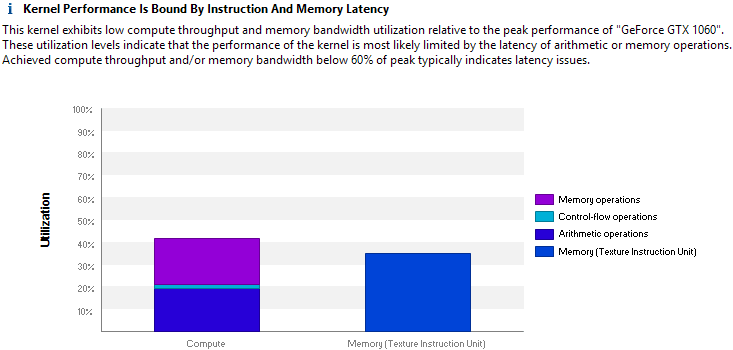
\includegraphics[width=\textwidth]{images/kernel_analysis_compute_force_nn_atomic.png}
    \caption{Atomic operations} \label{figure:kernel_analysis_compute_force_nn_atomic}
  \end{subfigure}\\ \bigskip
  \begin{subfigure}{.85\textwidth}
    \centering
    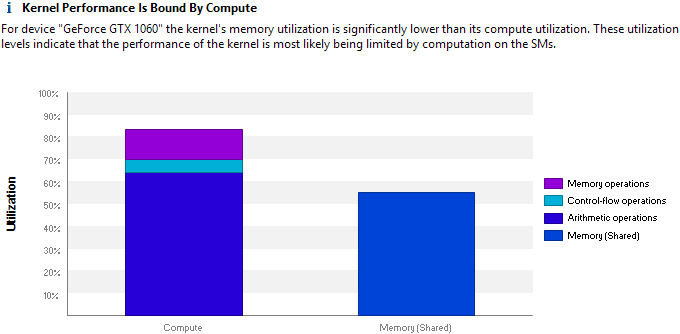
\includegraphics[width=\textwidth]{images/kernel_analysis_compute_force_nn_matrix.png}
    \caption{Matrix row summation} \label{figure:kernel_analysis_compute_force_nn_matrix}
  \end{subfigure}
  \caption{Kernel analysis of \texttt{compute\_force} on parallelise each body interaction method.}
\end{figure}

\subsection{Why N threads version is faster}
As shown in \cref{table:nn_version}, parallelising each body interaction (i.e. the force) is
significantly slower than parallelising each body. Justifications are given below:
\begin{enumerate}
  \item For atomic operations method, the performance loss increases exponentially when \textbf{N}
  increases. When \textbf{N} is large, a huge amount of time is spent on executing the force
  summation in serial due to the atomic section.

  \item The matrix row summation method is faster than atomic operations. In comparison with \(N\)
  thread version, this method requires an extra amount of computation. After calculating the forces
  between each body, it is still need to sum each row of the matrix to obtain the summation of
  forces for each body. This extra step is likely to have added a substantial amount of execution
  time.
\end{enumerate}

% ======================================================
\pagebreak
\section{Summary}
\renewcommand{\arraystretch}{1.3}
\begin{longtable}{|c|c|c|}
  \hline \endfirsthead \rowcolor{lightgray}
  Effective Optimisation & Avg. Speedup for \textbf{N} & Cumulative Speedup for \textbf{N} \\ \hline
  Baseline implementation    & 1.00 & 1.00  \\
  Block size from 32 to 256  & 1.31 & 1.31  \\
  Use CUDA \texttt{rsqrtf()} & 4.11 & 5.38  \\
  Read-only mem. for SoA     & 1.09 & 5.87  \\
  Shared memory              & 2.05 & \textbf{12.03} \\ \hline
  \caption{Summary of speedup achieved for \textbf{N} by effective optimisations.}
\end{longtable}
\renewcommand{\arraystretch}{1}

\renewcommand{\arraystretch}{1.3}
\begin{longtable}{|c|c|c|}
  \hline \endfirsthead \rowcolor{lightgray}
  Effective Optimisation & Avg. Speedup for \textbf{D} & Cumulative Speedup for \textbf{D} \\ \hline
  Baseline implementation    & 1.00 & 1.00 \\
  Block size from 32 to 256  & 1.61 & 1.61 \\
  Use CUDA \texttt{rsqrtf()} & 2.06 & 3.32 \\
  Read-only mem. for SoA     & 1.02 & 3.38 \\
  Shared memory              & 1.14 & \textbf{3.86} \\ \hline
  \caption{Summary of speedup achieved for \textbf{D} by effective optimisations.}
\end{longtable}
\renewcommand{\arraystretch}{1}

\begin{enumerate}
  \item 12.03x speedup on \textbf{N} and 3.86x speedup on \textbf{D} compared to the baseline
  implementation

  \item Kernel performance in only limited by single precision computations
\end{enumerate}

% ======================================================

\printbibliography[heading=bibintoc]

\end{document}
